\documentclass[12pt]{ociamthesis}  % default square logo
%\documentclass[12pt,beltcrest]{ociamthesis} % use old belt crest logo
%\documentclass[12pt,shieldcrest]{ociamthesis} % use older shield crest logo

%load any additional packages
\usepackage{amssymb}
\usepackage{tabularx}
\usepackage{multirow}
\usepackage{graphicx}
\usepackage[normalem]{ulem}
\useunder{\uline}{\ul}{}

%input macros (i.e. write your own macros file called mymacros.tex
%and uncomment the next line)
%\include{mymacros}

\title{Template Laporan Tingkat Akhir\\[1ex]     %your thesis title,
        Internship II atau Tugas Akhir}   %note \\[1ex] is a line break in the title

\author{Nama Mahasiswa}             %your name
\college{NPM\\[5ex]
In Partial Fulfilment of The Requirements for
The Degree of Applied Bachelor of Informatics Engineering}  %your college

%\renewcommand{\submittedtext}{change the default text here if needed}
\degree{Politeknik Pos Indonesia}     %the degree
\degreedate{Bandung 2018}         %the degree date

%end the preamble and start the document
\begin{document}

%this baselineskip gives sufficient line spacing for an examiner to easily
%markup the thesis with comments
\baselineskip=18pt plus1pt

%set the number of sectioning levels that get number and appear in the contents
\setcounter{secnumdepth}{3}
\setcounter{tocdepth}{3}


\maketitle                  % create a title page from the preamble info
\begin{dedication}
`Jika Kamu tidak dapat menahan lelahnya belajar, \\
Maka kamu harus sanggup menahan perihnya Kebodohan.'\\ 
~Imam Syafi'i~\\
\end{dedication}        % include a dedication.tex file
\begin{acknowledgements}
Pertama-tama kami panjatkan puji dan syukur kepada Allah SWT yang telah memberikan rahmat dan hidayah-Nya sehingga Buku Pedoman Tingkat Akhir ini dapat diselesaikan.
\end{acknowledgements}   % include an acknowledgements.tex file
\begin{abstract}
	Buku Pedoman ini dibuat dengan tujuan memberikan acuan, bagi mahasiswa Tingkat Akhir dan dosen
	Pembimbing. Pada intinya buku ini menjelaskan secara lengkap tentang Standar pengerjaan Intership  dan 
	Tugas Akhir
	di Program Studi D4 Teknik Informatika, dan juga mengatur mekanisme, teknik penulisan, serta
	penilaiannya.Dengan demikian diharapkan semua pihak yang terlibat dalam aktivitas Bimbingan Mahasiswa Tingkat Akhir
	berjalan lancar dan sesuai dengan standar.
\end{abstract}          % include the abstract

\begin{romanpages}          % start roman page numbering
\tableofcontents            % generate and include a table of contents
\listoffigures              % generate and include a list of figures
\end{romanpages}            % end roman page numbering

%now include the files of latex for each of the chapters etc
\begin{center}
  \textbf{Rekomendasi Penilaian}
\end{center}
Untuk memenuhi kelulusan Internship II \textbf{Syarat Kelulusan} :
\begin{enumerate}
  \item Dedikasi
  \item Produktifitas
  \item Integritas
  \item Disiplin
  \item Loyalitas
\end{enumerate}
Adapun \textbf{Syarat Khusus} :
\begin{enumerate}
  \item Kreatif Inisiatif
\end{enumerate}

\textbf{Keterangan}
\begin{enumerate}
\item Dedikasi
Berikut kategori penilaian dediskasi pada Tabel \ref{table:Dedikasi}
\begin{table}[!htbp]
\centering
\begin{tabular}{ |c|c|c|c|c|c|c|c|c|c| }
\hline
No. & Label & Nilai & Keterangan \\
\hline
1 & \textbf{TINGGI} & 3 & Full commit selama 5 hari kerja pada repositori buku informatika \\
\hline
2 & \textbf{SEDANG} & 2 & 4 hari kerja \\
\hline
3 & \textbf{RENDAH} & 1 & 0 s/d 3 hari kerja \\
\hline
\end{tabular}
\caption{Tabel Dedikasi}
\label{table:Dedikasi}
\end{table}

\item Produktifitas
Berikut kategori penilaian Profuktifitas pada Tabel \ref{table:Produktifitas}
\begin{table}[!htbp]
\centering
\begin{tabular}{ |c|c|c|c|c|c|c|c|c|c| }
\hline
No. & Label & Nilai & Keterangan \\
\hline
1 & \textbf{TINGGI} & 3 & Mengerjakan 5 pekerjaan harian \\
\hline
2 & \textbf{SEDANG} & 2 & Mengerjakan 4 pekerjaan harian \\
\hline
3 & \textbf{RENDAH} & 1 & Mengerjakan 0 s/d 3 pekerjaan harian \\
\hline
\end{tabular}
\caption{Tabel Produktifitas}
\label{table:Produktifitas}
\end{table}

\item Integritas
Berikut kategori penilaian Integritas pada Tabel \ref{table:Integritas}
\begin{table}[!htbp]
\centering
\begin{tabular}{ |c|c|c|c|c|c|c|c|c|c| }
\hline
No. & Label & Nilai & Keterangan \\
\hline
1 & \textbf{TINGGI} & 3 & Tidak ada penolakan pull request selama 5 hari kerja \\
\hline
2 & \textbf{SEDANG} & 2 & Ada 1 penolakan dalam 1 minggu \\
\hline
3 & \textbf{RENDAH} & 1 & Lebih dari satu penolakan dalam 1 minggu \\
\hline
\end{tabular}
\caption{Tabel Integritas}
\label{table:Integritas}
\end{table}

\item Disiplin
Berikut kategori penilaian Disiplin pada Tabel \ref{table:Disiplin}
\begin{table}[!htbp]
\centering
\begin{tabular}{ |c|c|c|c|c|c|c|c|c|c| }
\hline
No. & Label & Nilai & Keterangan \\
\hline
1 & \textbf{TINGGI} & 3 & Dalam satu minggu datang sebelum jam 9 pulang setelah jam 15 \\
\hline
2 & \textbf{SEDANG} & 2 & Ada satu hari telat \\
\hline
3 & \textbf{RENDAH} & 1 & Lebih dari satu hari telat \\
\hline
\end{tabular}
\caption{Tabel Disiplin}
\label{table:Disiplin}
\end{table}

\item Loyalitas
Berikut kategori penilaian Loyalitas pada Tabel \ref{table:Loyalitas}
\begin{table}[!htbp]
\centering
\begin{tabular}{ |c|c|c|c|c|c|c|c|c|c| }
\hline
No. & Label & Nilai & Keterangan \\
\hline
1 & \textbf{TINGGI} & 3 & Selama satu minggu Area kerja bersih tanpa ada debu dan indah, perangkat ada yang dijaga atau diperbaiki \\
\hline
2 & \textbf{SEDANG} & 2 & Ada satu hari area kerja tidak bersih dari debu dan berantakan, dan atau perangkat ada yang rusak \\
\hline
3 & \textbf{RENDAH} & 1 & Lebih dari satu hari, area kerja berantakan dan tidak ada perangkat yang jalan atau diperbaiki \\
\hline
\end{tabular}
\caption{Tabel Loyalitas}
\label{table:Loyalitas}
\end{table}

\item Kreatif dan Inisiatif
Berikut kategori penilaian Kreatif dan Inisiatif pada Tabel \ref{table:KnI}
\begin{table}[!htbp]
\centering
\begin{tabular}{ |c|c|c|c|c|c|c|c|c|c| }
\hline
No. & Label & Nilai & Keterangan \\
\hline
1 & \textbf{TINGGI} & 3 & Menjadi tentor dengan jumlah peserta minimal 10 orang berbayar atau bersponsor \\
\hline
2 & \textbf{SEDANG} & 2 & Menjadi tentor dengan jumlh peserta minimal 5 orang berbayar atau bersponsor \\
\hline
3 & \textbf{RENDAH} & 1 & Selain kategori diatas \\
\hline
\end{tabular}
\caption{Tabel Kreatif dan Inisiatif}
\label{table:KnI}
\end{table}
\end{enumerate}
\textbf {Ketentuan}
\begin{enumerate}
  \item Nilai minimal syarat umum adalah 13 dari rata2 minimall 20 minggu. apabila kurang dari 13 maka bisa menambah lagi waktu intership sesuai dengan kebutuhan nilai minimum.
  \item Syarat khusus bisa diselenggarakan minimal sekali dengan minimal nilai sedang
\end{enumerate}
\textbf{Penilaian}
\par Tabel \ref{table:Penilaian} adalah data penilaian mahasiswa Internship II atau TA.
\begin{table}[!htbp]
\centering
\begin{tabular}{ |c|c|c|c|c|c|c|c|c|c| }
\hline
 &  &  &  &  \\
\hline
 &  &  &  &  \\
\hline
 &  &  &  &  \\
\hline
 &  &  &  &  \\
\hline
 &  &  &  &  \\
\hline
 &  &  &  &  \\
\hline
 &  &  &  &  \\
\hline
 &  &  &  &  \\
\hline
 &  &  &  &  \\
\hline
 &  &  &  &  \\
\hline
 &  &  &  &  \\
\hline
 &  &  &  &  \\
\hline
 &  &  &  &  \\
\hline
 &  &  &  &  \\
\hline
 &  &  &  &  \\
\hline
 &  &  &  &  \\
\hline
 &  &  &  &  \\
\hline
 &  &  &  &  \\
\hline
 &  &  &  &  \\
\hline
 &  &  &  &  \\
\hline
\end{tabular}
\caption{Tabel Penilaian}
\label{table:Penilaian}
\end{table}
\chapter{Dzikri Ahmad Ghifari/1144077}
\begin{enumerate}
\item \textbf{Tugas Harian tanggal 17/01/2019}
\begin{enumerate}
\item Membersihkan ruang IRC
\item Diskusi mengenai penataan ulang ruang IRC
\end{enumerate}

\item \textbf{Tugas Harian tanggal 18/01/2019}
\begin{enumerate}
\item Membersihkan ruang IRC
\item Diskusi mengenai rancangan ruang IRC
\item Diskusi mengenai barang yang harus ditambahkan di ruang IRC
\item Membuat artikel untuk bahan majalah D4 TI
\end{enumerate}

\item \textbf{Tugas Harian tanggal 21/01/2019}
\begin{enumerate}
\item Mencari artikel untuk bahan majalah
\item Diskusi tentang perancangan ruang sidang di IRC
\end{enumerate}

\item \textbf{Tugas Harian tanggal 30/02/2019}
\begin{enumerate}
\item Mendata buku yang akan dipindahkan ke IRC
\end{enumerate}

\item \textbf{Tugas Harian tanggal 31/01/2019}
\begin{enumerate}
\item Memberi label pada buku untuk IRC
\item Memindahkan buku sumbangan ke IRC
\end{enumerate}

\item \textbf{Tugas Harian tanggal 01/02/2019}
\begin{enumerate}
\item Praktek github dengan Pak Rolly Maulana Awangga 
\end{enumerate}

\item \textbf{Tugas Harian tanggal 06/02/2019}
\begin{enumerate}
\item Membuat video pesan, kesan dan kritik untuk IRC
\end{enumerate}

\item \textbf{Tugas Harian tanggal 18/02/2019}
\begin{enumerate}
\item Memperhatikan tingkat 3 presentasi
\item Mengoreksi laporan tingkat 3 yang presentasi
\item Memeriksa revisian tutorial class diagram adik tingkat
\end{enumerate}

\item \textbf{Tugas Harian tanggal 25/02/2019}
\begin{enumerate}
\item Masuk Kelas Pemrograman III
\item Menginstal python, anaconda
\item Menambah materi udemy (commit 8b5991b08ef04a0c1581f5976017e7eab865c856)
\item Menambah materi di GIS2019 (commit f1535f03dd64c09ddba50f68371ec04b878846e9, commit 0ff764471c1cefd7e6b20d81027d7d810c1343d5, commit c054dcbfa03e9a2d9ef56f3302d8f0854840d758)
\item Memeriksa tugas Pemrograman III kelas 2b (1174034 Ichsan Hizman Hardy, 1174050 Dika Sukma Pradana, 1174042 Faisal Najib Abdullah, 1174035 Luthfi Muhammad Nabil, 1174040 Hagan Rowlenstino, 1174043 Irvan Rizkiansyah, 1174063 Muhamad Iqbal Panggabean, 1174057 Alit fajar Kurniawan, 1174059 Kevin Natanael Nainggolan)
\end{enumerate}

\textbf{Dedikasi}
\begin{enumerate} 
\item  Menambah materi di GIS2019 (commit f1535f03dd64c09ddba50f68371ec04b878846e9, commit 0ff764471c1cefd7e6b20d81027d7d810c1343d5, commit c054dcbfa03e9a2d9ef56f3302d8f0854840d758)
\end{enumerate}

\textbf{Produktifitas}
\begin{enumerate}
\item Masuk Kelas Pemrograman III
\item Menginstal python, anaconda
\item Menambah materi udemy (commit 8b5991b08ef04a0c1581f5976017e7eab865c856
\item Menambah materi di GIS2019 (commit f1535f03dd64c09ddba50f68371ec04b878846e9, commit 0ff764471c1cefd7e6b20d81027d7d810c1343d5, commit c054dcbfa03e9a2d9ef56f3302d8f0854840d758)
\item Memeriksa tugas Pemrograman III kelas 2b (1174034 Ichsan Hizman Hardy, 1174050 Dika Sukma Pradana, 1174042 Faisal Najib Abdullah, 1174035 Luthfi Muhammad Nabil, 1174040 Hagan Rowlenstino, 1174043 Irvan Rizkiansyah, 1174063 Muhamad Iqbal Panggabean, 1174057 Alit fajar Kurniawan, 1174059 Kevin Natanael Nainggolan)
\end{enumerate}

\textbf{Integritas}
\begin{enumerate}
\item able to merge/has no conflict
\end{enumerate}

\textbf{Disiplin}
\begin{enumerate}
\item Jam Masuk : 08.40
\item Jam Keluar : 15.30
\end{enumerate}

\textbf{Loyalitas}
\begin{enumerate}
\item Mengecek AC saat datang dan pulang dari IRC
\item Merapihkan meja dan kursi saat pulang dari IRC
\item Merapihkan CPU ke lemari
\item Merapihkan banner ke lemari
\item Menjaga peralatan yang ada di IRC  
\end{enumerate}

\item \textbf{Tugas Harian tanggal 26/02/2019}
\begin{enumerate}
\item Masuk kelas Kecerdasan Buatan
\item Membuat repository tugas kecerdasan buatan kelas 3c
\item Menginput nilai tugas Pemrograman III kelas 2b
\item Menambah materi GIS 2019, commit d97e9474087a3faca296fef82e9e7503345ac45e
\end{enumerate}

\textbf{Dedikasi}
\begin{enumerate}
\item Menambah materi GIS 2019, commit d97e9474087a3faca296fef82e9e7503345ac45e
\end{enumerate}

\textbf{Produktifitas}
\begin{enumerate}
\item Masuk kelas Kecerdasan Buatan
\item Membuat repository tugas kecerdasan buatan kelas 3c
\item Menginput nilai tugas Pemrograman III kelas 2b
\item Menambah materi GIS 2019, commit d97e9474087a3faca296fef82e9e7503345ac45e
\end{enumerate}

\textbf{Integritas}
\begin{enumerate}
\item able to merge/has no conflict
\end{enumerate}

\textbf{Disiplin}
\begin{enumerate}
\item Jam Masuk : 08.40
\item Jam Keluar : 15.30
\end{enumerate}

\textbf{Loyalitas}
\begin{enumerate}
\item Mengecek AC saat datang dan pulang dari IRC
\item Merapihkan kursi saat pulang dari IRC
\item Menjaga peralatan yang ada di IRC
\end{enumerate}

\item \textbf{Tugas Harian tanggal 27/02/2019}
\begin{enumerate}
\item Mangecek tugas kecerdasan buatan kelas 3c
\item Menginput nilai tugas kecerdasan buatan kelas 3c
\item Memberikan arahan dan hukuman bagi mahasiswa yang tidak melakukan pull request, tidak membenarkan conflict dan tidak mengerjakan tugas Pemrograman III kelas 2b
\item Menginput nilai tugas Pemrograman III kelas 2b (1174034 Ichsan Hizman Hardy, 1174050 Dika Sukma Pradana, 1174042 Faisal Najib Abdullah, 1174035 Luthfi Muhammad Nabil, 1174040 Hagan Rowlenstino, 1174043 Irvan Rizkiansyah, 1174063 Muhamad Iqbal Panggabean, 1174057 Alit fajar Kurniawan, 1174059 Kevin Natanael Nainggolan)
\item Menambah materi GIS 2019, commit d97e9474087a3faca296fef82e9e7503345ac45e
\item Menandatangani acc tutorial membuat class diagram (Ajis Trigunawan 1164031 dan Wildan Khaustara W 1164058)
\item Memeriksa dan memberi revisian jurnal projek II Ajis Trigunawan 1164031
\end{enumerate}

\textbf{Dedikasi}
\begin{enumerate}
\item Menambah materi GIS 2019, commit d97e9474087a3faca296fef82e9e7503345ac45e
\end{enumerate}

\textbf{Produktifitas}
\begin{enumerate}
\item Masuk kelas Kecerdasan Buatan
\item Membuat repository tugas kecerdasan buatan kelas 3c
\item Menginput nilai tugas Pemrograman III kelas 2b (1174034 Ichsan Hizman Hardy, 1174050 Dika Sukma Pradana, 1174042 Faisal Najib Abdullah, 1174035 Luthfi Muhammad Nabil, 1174040 Hagan Rowlenstino, 1174043 Irvan Rizkiansyah, 1174063 Muhamad Iqbal Panggabean, 1174057 Alit fajar Kurniawan, 1174059 Kevin Natanael Nainggolan)
\item Menambah materi GIS 2019, commit d97e9474087a3faca296fef82e9e7503345ac45e
\item Menandatangani acc tutorial membuat class diagram (Ajis Trigunawan 1164031 dan Wildan Khaustara W 1164058)
\item Memeriksa dan memberi revisian jurnal projek II Ajis Trigunawan 1164031
\end{enumerate}

\textbf{Integritas}
\begin{enumerate}
\item able to merge/has no conflict
\end{enumerate}

\textbf{Disiplin}
\begin{enumerate}
\item Jam Masuk : 08.40
\item Jam Keluar : 15.30
\end{enumerate}

\textbf{Loyalitas}
\begin{enumerate}
\item Mengecek AC saat datang dan pulang dari IRC
\item Merapihkan kursi saat pulang dari IRC
\item Menjaga peralatan yang ada di IRC
\end{enumerate}

\item \textbf{Tugas Harian tanggal 27/02/2019}
\begin{enumerate}
\item Mangecek tugas kecerdasan buatan kelas 3c (Andi Muh Aslam 1164064 dan Aip Suprapto Munari 1164063)
\item Menginput nilai tugas kecerdasan buatan kelas 3c (Andi Muh Aslam 1164064 dan Aip Suprapto Munari 1164063)
\item Memberikan arahan dan hukuman bagi mahasiswa yang tidak melakukan pull request, tidak membenarkan conflict dan tidak mengerjakan tugas Pemrograman III kelas 2b
\item Menambah gambar pada Materi GIS (menambahkan gambar \#11) 
\end{enumerate}

\textbf{Dedikasi}
\begin{enumerate}
\item Menambah gambar pada Materi GIS (menambahkan gambar \#11) 
\end{enumerate}

\textbf{Produktifitas}
\begin{enumerate}
\item Mangecek tugas kecerdasan buatan kelas 3c (Andi Muh Aslam 1164064 dan Aip Suprapto Munari 1164063)
\item Menginput nilai tugas kecerdasan buatan kelas 3c (Andi Muh Aslam 1164064 dan Aip Suprapto Munari 1164063)
\item Memberikan arahan dan hukuman bagi mahasiswa yang tidak melakukan pull request, tidak membenarkan conflict dan tidak mengerjakan tugas Pemrograman III kelas 2b
\item Menambah gambar pada Materi GIS (menambahkan gambar \#11) 
\end{enumerate}

\textbf{Integritas}
\begin{enumerate}
\item able to merge/has no conflict
\end{enumerate}

\textbf{Disiplin}
\begin{enumerate}
\item Jam Masuk : 08.40
\item Jam Keluar : 15.30
\end{enumerate}

\textbf{Loyalitas}
\begin{enumerate}
\item Mengecek AC saat datang dan pulang dari IRC
\item Merapihkan kursi saat pulang dari IRC
\item Menjaga peralatan yang ada di IRC
\end{enumerate}


\item \textbf{Tugas Harian tanggal 28/02/2019}
\begin{enumerate}
\item Evaluasi mingguan dengan Pak Rolly Maulana Awangga
\item Menilai hasil UAS kelas 1C, 3A dan 3C
\item Menata ulang ruang IRC
\item Memeriksa tugas kelas Kecerdasan Buatan 3C Andi Muh Aslam 1164064, hari2 \#3 dan  Aip Suprapto Munari 1164063  (tugas masih conflict)
\item Menginput nilai tugas Kecerdasan Buatan kelas 3C Andi Muh Aslam 1164064 dan Aip Suprapto Munari 1164063 
\item Menambah materi sumber sumber data geospasial \#13
\end{enumerate}

\textbf{Dedikasi}
\begin{enumerate}
\item Menambah materi sumber sumber data geospasial \#13
\end{enumerate}

\textbf{Produktifitas}
\begin{enumerate}
\item Evaluasi mingguan dengan Pak Rolly Maulana Awangga
\item Menilai hasil UAS kelas 1C, 3A dan 3C
\item Menata ulang ruang IRC
\item Memeriksa tugas kelas Kecerdasan Buatan 3C Andi Muh Aslam 1164064, hari2 \#3 dan  Aip Suprapto Munari 1164063  (tugas masih conflict)
\item Menginput nilai tugas Kecerdasan Buatan kelas 3C Andi Muh Aslam 1164064 dan Aip Suprapto Munari 1164063 
\end{enumerate}

\textbf{Integritas}
\begin{enumerate}
\item able to merge/has no conflict
\end{enumerate}

\textbf{Disiplin}
\begin{enumerate}
\item Jam Masuk : 08.40
\item Jam Keluar : 17.30
\end{enumerate}

\textbf{Loyalitas}
\begin{enumerate}
\item Mengecek AC saat datang dan pulang dari IRC
\item Merapihkan kursi saat pulang dari IRC
\item Menjaga peralatan yang ada di IRC
\item Mengatur ulang ruang IRC 
\end{enumerate}

\item \textbf{Tugas Harian tanggal 01/03/2019}
\begin{enumerate} 
\item Melakukan pre test TOEFL 
\item Memberi tahu kelas 3B untuk mencantumkan sitasi dan sumber di daftar pustaka mengenai materi GIS
\item menambah materi dan gambar mengenai sumber sumber data geospasial \#16
\end{enumerate}

\textbf{Dedikasi}
\begin{enumerate}
\item menambah materi dan gambar mengenai sumber sumber data geospasial \#16
\end{enumerate}

\textbf{Produktifitas}
\begin{enumerate}
\item Melakukan pre test TOEFL 
\item Memberi tahu kelas 3B untuk mencantumkan sitasi dan sumber di daftar pustaka mengenai materi GIS
\item menambah materi dan gambar mengenai sumber sumber data geospasial \#16
\end{enumerate}

\textbf{Integritas}
\begin{enumerate}
\item able to merge/has no conflict
\end{enumerate}


\textbf{Disiplin}
\begin{enumerate}
\item Jam Masuk : 08.40
\item Jam Keluar : 11.40 (Dikarenakan ada sosialisasi INTERNSHIP II)
\end{enumerate}


\textbf{Loyalitas}
\begin{enumerate}
\item Mengecek AC saat datang dan pulang dari IRC
\item Menjaga peralatan yang ada di IRC
\item Merapihkan kursi setelah pulamg dari IRC
\item Mengelap meja pribadi
\item Menyapu dan merapihkan area sidang IRC
\item Membersihkan lemari buku 
\end{enumerate}

\item \textbf{Tugas Harian tanggal 04/03/2019}
\begin{enumerate}
\item Menambah gambar dan materi mengenai sumber sumber data geospasial \#17
\item Masuk kelas Pemrograman 3 
\item Diskusi mengenai INTERNSHIP II bersama Bapak Rolly Maulana Awangga
\item Membuat orgnanisasi INTERNSHIPD4TI di github
\item Kontribusi pada repository PPK (template \#1, merapihkan dan menambah contoh laporan harian dan mingguan \#8)
\item Menambah materi deep learning computer vision \#3
\item Menilai presentasi Rizal Ramadhan D4 TI 1c 
\item Membersihkan meja pribadi
\item Membersihkan area sidang 
\end{enumerate}

\textbf{Dedikasi}
\begin{enumerate}
\item Menambah gambar dan materi mengenai sumber sumber data geospasial \#17
\item Kontribusi pada repository PPK (template \#1, merapihkan dan menambah contoh laporan harian dan mingguan \#8)
\item Menambah materi deep learning computer vision \#3
\end{enumerate}

\textbf{Produktifitas}
\begin{enumerate}
\item Menambah gambar dan materi mengenai sumber sumber data geospasial \#17
\item Masuk kelas Pemrograman 3 
\item Diskusi mengenai INTERNSHIP II bersama Bapak Rolly Maulana Awangga
\item Membuat orgnanisasi INTERNSHIPD4TI di github
\item Kontribusi pada repository PPK (template \#1, merapihkan dan menambah contoh laporan harian dan mingguan \#8)
\item Menambah materi deep learning computer vision \#3
\item Menilai presentasi Rizal Ramadhan D4 TI 1c 
\item Membersihkan meja pribadi
\item Menyapu dan merapihkan area sidang 
\end{enumerate}

\textbf{Integritas}
\begin{enumerate}
\item able to merge/has no conflict
\end{enumerate}


\textbf{Disiplin}
\begin{enumerate}
\item Jam Masuk : 08.40
\item Jam Keluar : 17.40
\end{enumerate}


\textbf{Loyalitas}
\begin{enumerate}
\item Mengecek AC saat datang dan pulang dari IRC
\item Menjaga peralatan yang ada di IRC
\item Merapihkan kursi setelah pulamg dari IRC
\item Mengelap meja pribadi
\item Menyapu dan merapihkan area sidang IRC
\item Membersihkan meja pribadi
\end{enumerate}

\item \textbf{Tugas Harian tanggal 05/03/2019}
\begin{enumerate}
\item Masuk kelas Kecerdasan Buatan 
\item Merapihkan Panduan Peningkatan Kompetensi(merapihkan \#10)
\item Menambah gambar untuk materi sumber-sumber data geospasial, menambah materi mengenai pengenalan sistem informasi geografis \#18
\item Memeriksa dan memerge praktek Pemrograman III kelas 2B(Faisal Najib Abdullah 1174042, Muhammad Iqbal Panggabean 1174063, Hagan Rowlenstino 1174040, Luthfi Muhammad Nabil 1174035, Irvan Rizkiansyah 1174043, Dika Sukma Pradana 1174050, Fathir (conflict), Yusniar Nur Syarif Sidiq 1164089, Ichsan Hizman Hardy 1174034, Alit Fajar Kurniawan 1174057, Kevin Natanael Nainggolan 1174059, Mhd Zulfikar Akram Nasution 1164081(conflict), Muhammad Afra Faris 1174041 (telat meresolve conflict), Rangga Putra Ramdhani 1174056(conflict))
\item Membimbing anak kelas 2B mengenai penggunaan github
\item Menyapu area sidang IRC
\item Membeersihkan meja kerja 
\end{enumerate}

\textbf{Dedikasi}
\begin{enumerate}
\item Merapihkan Panduan Peningkatan Kompetensi(merapihkan \#10)
\item Menambah gambar untuk materi sumber-sumber data geospasial, menambah materi mengenai pengenalan sistem informasi geografis \#18
\end{enumerate}

\textbf{Produktifitas}
\begin{enumerate}
\item Masuk kelas Kecerdasan Buatan 
\item Merapihkan Panduan Peningkatan Kompetensi(merapihkan \#10)
\item Menambah gambar untuk materi sumber-sumber data geospasial, menambah materi mengenai pengenalan sistem informasi geografis \#18
\item Memeriksa dan memerge praktek Pemrograman III kelas 2B(Faisal Najib Abdullah 1174042, Muhammad Iqbal Panggabean 1174063, Hagan Rowlenstino 1174040, Luthfi Muhammad Nabil 1174035, Irvan Rizkiansyah 1174043, Dika Sukma Pradana 1174050, Fathir (conflict), Yusniar Nur Syarif Sidiq 1164089, Ichsan Hizman Hardy 1174034, Alit Fajar Kurniawan 1174057, Kevin Natanael Nainggolan 1174059, Mhd Zulfikar Akram Nasution 1164081(conflict), Muhammad Afra Faris 1174041 (telat meresolve conflict), Rangga Putra Ramdhani 1174056(conflict))
\item Membimbing anak kelas 2B mengenai penggunaan github
\item Menyapu area sidang IRC
\item Membeersihkan meja kerja 
\end{enumerate}

\textbf{Integritas}
\begin{enumerate}
\item able to merge/has no conflict
\end{enumerate}


\textbf{Disiplin}
\begin{enumerate}
\item Jam Masuk : 08.30
\item Jam Keluar : 17.40
\end{enumerate}


\textbf{Loyalitas}
\begin{enumerate}
\item Mengecek AC saat datang dan pulang dari IRC
\item Menjaga peralatan yang ada di IRC
\item Merapihkan kursi setelah pulamg dari IRC
\item Mengelap meja pribadi
\item Menyapu dan merapihkan area sidang IRC
\item Membersihkan meja pribadi
\end{enumerate}

\item \textbf{Tugas Harian tanggal 06/03/2019}
\begin{enumerate}
\item Menambah materi mengenai pengertian GIS menurut para ahli \#20
\item Memeriksa tugas kecerdasan buatan kelas 3c (Andi Muh Aslam 1164064 dan Aip Suprapto Munari 1164063) bagian pertama untuk chapter 2
\item Memeriksa jurnal Eko Cahyono Putro dan Nur Arkhamia Batubara kelas D4 TI 33B
\item Menginput nilai kecerdasan buatan kelas 3c (Andi Muh Aslam 1164064 dan Aip Suprapto Munari 1164063) bagian pertama untuk chapter 2
\item Membersihkan dan merapihkan area sidang IRC
\item Menyapu area sidang IRC
\item Merapihkan kursi di area sidang IRC
\end{enumerate}

\textbf{Dedikasi}
\begin{enumerate}
\item Menambah materi mengenai pengertian GIS menurut para ahli \#20
\end{enumerate}

\textbf{Produktifitas}
\begin{enumerate}
\item Menambah materi mengenai pengertian GIS menurut para ahli \#20
\item Memeriksa tugas kecerdasan buatan kelas 3c (Andi Muh Aslam 1164064 dan Aip Suprapto Munari 1164063) bagian pertama pada chapter2
\item Memeriksa jurnal Eko Cahyono Putro dan Nur Arkhamia Batubara kelas D4 TI 33B
\item Menginput nilai kecerdasan buatan kelas 3c (Andi Muh Aslam 1164064 dan Aip Suprapto Munari 1164063)
\item Membersihkan dan merapihkan area sidang IRC
\item Menyapu area sidang IRC
\item Merapihkan kursi di area sidang IRC
\end{enumerate}

\textbf{Integritas}
\begin{enumerate}
\item able to merge/has no conflict
\end{enumerate}


\textbf{Disiplin}
\begin{enumerate}
\item Jam Masuk : 08.30
\item Jam Keluar : 18.00
\end{enumerate}


\textbf{Loyalitas}
\begin{enumerate}
\item Mengecek AC saat datang dan pulang dari IRC
\item Menjaga peralatan yang ada di IRC
\item Merapihkan kursi setelah pulamg dari IRC
\item Menyapu dan membersihkan area sidang IRC
\item Membersihkan meja pribadi
\end{enumerate}

\item \textbf{Tugas Harian tanggal 08/03/2019}
\begin{enumerate}
\item Menambah materi mengenai pengenalan sistem informasi geografis \#21 pada repository GIS2019
\item Menambah materi alat pendeteksi banjir \#10 pada pada repository IoT 
\item Memeriksa tugas mata kuliah kecerdasan buatan kelas 3c (Andi Muh Aslam 1164064 dan Aip Suprapto Munari 1164063) bagian kedua pada chapter2
\item Menyapu ruang IRC
\item Membersihkan meja kerja pribadi di IRC
\end{enumerate}

\textbf{Dedikasi}
\begin{enumerate}
\item Menambah materi mengenai pengenalan sistem informasi geografis \#21 pada repository GIS2019
\item Menambah materi alat pendeteksi banjir \#10 pada pada repository IoT 
\end{enumerate}

\textbf{Produktifitas}
\begin{enumerate}
\item Menambah materi mengenai pengenalan sistem informasi geografis \#21 pada repository GIS2019
\item Menambah materi alat pendeteksi banjir \#10 pada pada repository IoT 
\item Memeriksa tugas mata kuliah kecerdasan buatan kelas 3c (Andi Muh Aslam 1164064 dan Aip Suprapto Munari 1164063) bagian kedua pada chapter2
\item Menyapu ruang IRC
\item Membersihkan meja kerja pribadi di IRC
\end{enumerate}

\textbf{Integritas}
\begin{enumerate}
\item able to merge/has no conflict
\end{enumerate}


\textbf{Disiplin}
\begin{enumerate}
\item Jam Masuk : 08.30
\item Jam Keluar : 16.40
\end{enumerate}


\textbf{Loyalitas}
\begin{enumerate}
\item Mengecek AC saat datang dan pulang dari IRC
\item Menjaga peralatan yang ada di IRC
\item Merapihkan kursi setelah pulamg dari IRC
\item Menyapu dan membersihkan area sidang IRC
\item Membersihkan meja pribadi
\item Mencuci gelas
\end{enumerate}

\item \textbf{Tugas Harian tanggal 11/03/2019}
\begin{enumerate}
\item Menambah materi mengenai pengenalan sistem informasi geografis dan menginput chapter tipe tipe data geospasial \#23
\item Masuk kelas Pemrograman III
\item Memeriksa Quiz I Mata Kuliah Pemrograman III kelas 2b (Irvan Rizkiansyah 1174043, Fathi Rabbani 1164074, Yusniar Nur Syarif Sidiq 1164089, Muhammad Afra Faris 1174041, Salwa Tania 1174047, Teddy Gidean Manik 1174038, Rangga Putra Ramadhan 1174056)
\item Menginput nilai Quiz I Mata Kuliah Pemrograman III kelas 2b (Irvan Rizkiansyah 1174043, Fathi Rabbani 1164074, Yusniar Nur Syarif Sidiq 1164089, Muhammad Afra Faris 1174041, Salwa Tania 1174047, Teddy Gidean Manik 1174038, Rangga Putra Ramadhan 1174056)
\item Menyapu area sidang IRC
\item Merapihkan kursi setelah jam pulang 
\end{enumerate}

\textbf{Dedikasi}
\begin{enumerate}
\item Menambah materi mengenai pengenalan sistem informasi geografis dan menginput chapter tipe tipe data geospasial \#23
\end{enumerate}

\textbf{Produktifitas}
\begin{enumerate}
\item Menambah materi mengenai pengenalan sistem informasi geografis dan menginput chapter tipe tipe data geospasial \#23
\item Masuk kelas Pemrograman III
\item Memeriksa Quiz I Mata Kuliah Pemrograman III kelas 2b (Irvan Rizkiansyah 1174043, Fathi Rabbani 1164074, Yusniar Nur Syarif Sidiq 1164089, Muhammad Afra Faris 1174041, Salwa Tania 1174047, Teddy Gidean Manik 1174038, Rangga Putra Ramadhan 1174056)
\item Menginput nilai Quiz I Mata Kuliah Pemrograman III kelas 2b (Irvan Rizkiansyah 1174043, Fathi Rabbani 1164074, Yusniar Nur Syarif Sidiq 1164089, Muhammad Afra Faris 1174041, Salwa Tania 1174047, Teddy Gidean Manik 1174038, Rangga Putra Ramadhan 1174056)
\item Menyapu area sidang IRC
\item Merapihkan kursi setelah jam pulang 
\end{enumerate}

\textbf{Integritas}
\begin{enumerate}
\item able to merge/has no conflict
\end{enumerate}


\textbf{Disiplin}
\begin{enumerate}
\item Jam Masuk : 08.35
\item Jam Keluar : 16.20
\end{enumerate}


\textbf{Loyalitas}
\begin{enumerate}
\item Mengecek AC saat datang dan pulang dari IRC
\item Menjaga peralatan yang ada di IRC
\item Merapihkan kursi setelah pulamg dari IRC
\item Menyapu dan membersihkan area sidang IRC
\item Membersihkan meja pribadi
\end{enumerate}


\item \textbf{Tugas Harian tanggal 12/03/2019}
\begin{enumerate}
\item Menambah materi mengenai pengenalan sistem informasi geografis \#24
\item Memerge tugas chapter 3 mata kuliah Pemrograman III kelas 2b pada hari senin malam hingga hari selasa pagi jam 04.00
\item Memeriksa ulang nilai Quiz I Mata Kuliah Pemrograman III kelas 2b (Irvan Rizkiansyah 1174043, Fathi Rabbani 1164074, Yusniar Nur Syarif Sidiq 1164089, Muhammad Afra Faris 1174041, Salwa Tania 1174047, Teddy Gidean Manik 1174038, Rangga Putra Ramadhan 1174056)
\item Merubah nilai Quiz I Mata Kuliah Pemrograman III kelas 2b (Irvan Rizkiansyah 1174043, Fathi Rabbani 1164074, Yusniar Nur Syarif Sidiq 1164089, Muhammad Afra Faris 1174041, Salwa Tania 1174047, Teddy Gidean Manik 1174038, Rangga Putra Ramadhan 1174056)
\item Memeriksa Tugas Mata Kuliah pemrograman III kelas 2b
\item Merangkum materi \#26 GIS2019
\item Menyapu area sidang IRC
\item Membersihkan meja pribadi dan area belakang IRC
\item Merapihkan kursi setelah jam pulang 
\end{enumerate}

\textbf{Dedikasi}
\begin{enumerate}
\item Menambah materi mengenai pengenalan sistem informasi geografis \#24
\item Merangkum materi \#26 GIS2019
\end{enumerate}

\textbf{Produktifitas}
\begin{enumerate}
\item Menambah materi mengenai pengenalan sistem informasi geografis \#24
\item Memerge tugas chapter 3 mata kuliah Pemrograman III kelas 2b pada hari senin malam hingga hari selasa pagi jam 04.00
\item Memeriksa ulang nilai Quiz I Mata Kuliah Pemrograman III kelas 2b (Irvan Rizkiansyah 1174043, Fathi Rabbani 1164074, Yusniar Nur Syarif Sidiq 1164089, Muhammad Afra Faris 1174041, Salwa Tania 1174047, Teddy Gidean Manik 1174038, Rangga Putra Ramadhan 1174056)
\item Merubah nilai Quiz I Mata Kuliah Pemrograman III kelas 2b (Irvan Rizkiansyah 1174043, Fathi Rabbani 1164074, Yusniar Nur Syarif Sidiq 1164089, Muhammad Afra Faris 1174041, Salwa Tania 1174047, Teddy Gidean Manik 1174038, Rangga Putra Ramadhan 1174056)
\item Memeriksa Tugas Mata Kuliah Pemrograman III kelas 2b
\item Merangkum materi \#26 GIS2019
\item Menyapu area sidang IRC
\item Membersihkan meja pribadi dan area belakang IRC
\item Merapihkan kursi setelah jam pulang 
\end{enumerate}

\textbf{Integritas}
\begin{enumerate}
\item able to merge/has no conflict
\end{enumerate}


\textbf{Disiplin}
\begin{enumerate}
\item Jam Masuk : 08.35
\item Jam Keluar : 16.30
\end{enumerate}


\textbf{Loyalitas}
\begin{enumerate}
\item Mengecek AC saat datang dan pulang dari IRC
\item Menjaga peralatan yang ada di IRC
\item Merapihkan kursi setelah pulamg dari IRC
\item Menyapu dan membersihkan area sidang IRC
\item Membersihkan meja pribadi
\item Membersihkan area belakang IRC
\item Mencuci gelas
\end{enumerate}


\item \textbf{Tugas Harian tanggal 13/03/2019}
\begin{enumerate}
\item Merangkum materi \#27
\item Memeriksa tugas chapter 3 kelas 2b (IrvanRizkiansyah1174043, Luthfi Muhammad Nabil 1174035, Rangga Putra Ramdhan 1174056, Faisal Najib Abdullah 1174042, Mhd Zulfikar Akram Nasution 1164081)
\item Menginput nilai tugas chapter 3 kelas 2b (IrvanRizkiansyah1174043, Luthfi Muhammad Nabil 1174035, Rangga Putra Ramdhan 1174056, Faisal Najib Abdullah 1174042, Mhd Zulfikar Akram Nasution 1164081)
\item Menyapu area sidang IRC
\item Membersihkan meja pribadi dan area belakang IRC
\item Merapihkan kursi setelah jam pulang 
\end{enumerate}

\textbf{Dedikasi}
\begin{enumerate}
\item Merangkum materi \#27
\end{enumerate}

\textbf{Produktifitas}
\begin{enumerate}
\item Merangkum materi \#27
\item Memeriksa tugas chapter 3 kelas 2b (IrvanRizkiansyah1174043, Luthfi Muhammad Nabil 1174035, Rangga Putra Ramdhan 1174056, Faisal Najib Abdullah 1174042, Mhd Zulfikar Akram Nasution 1164081)
\item Menginput nilai tugas chapter 3 kelas 2b (IrvanRizkiansyah1174043, Luthfi Muhammad Nabil 1174035, Rangga Putra Ramdhan 1174056, Faisal Najib Abdullah 1174042, Mhd Zulfikar Akram Nasution 1164081)
\item Menyapu area sidang IRC
\item Membersihkan meja pribadi dan area belakang IRC
\item Merapihkan kursi setelah jam pulang 
\end{enumerate}

\textbf{Integritas}
\begin{enumerate}
\item able to merge/has no conflict
\end{enumerate}

\textbf{Disiplin}
\begin{enumerate}
\item Jam Masuk : 08.35
\item Jam Keluar : 16.30
\end{enumerate}

\textbf{Loyalitas}
\begin{enumerate}
\item Mengecek AC saat datang dan pulang dari IRC
\item Menjaga peralatan yang ada di IRC
\item Merapihkan kursi setelah pulamg dari IRC
\item Menyapu dan membersihkan area sidang IRC
\item Membersihkan meja pribadi
\item Membersihkan area belakang IRC
\item Mencuci gelas
\end{enumerate}

\item \textbf{Tugas Harian tanggal 14/03/2019}
\begin{enumerate}
\item Menambah materi mengenai pengenalan sistem informasi geografis \#30
\item Diskusi mengenai barang barang yang akan ditambahkan ke IRC
\item Masuk ke kelas 3c Mata Kuliah Kecerdasan Buatan 
\item Melakukan latihan dasar menggunakan gitlab
\item Memeriksa jurnal IMPLEMENTASAI BOOYER MOORE PADA APLIKASI PENCARIAN DAN PENGUMUMAN BARANG HILANG (Ajis Trigunawan 1164031 dan Wildan Khaustara W 1164058)
\item Memberikan arahan kepada Tommy dan Yoshi mengenai tugas di github bukuinformatika, dasar dasar latex dan perintah perintah dasar pada gitbash 
\item Menyapu area sidang IRC
\item Membersihkan meja pribadi dan area belakang IRC
\item Merapihkan kursi setelah jam pulang 
\end{enumerate}

\textbf{Dedikasi}
\begin{enumerate}
\item Menambah materi mengenai pengenalan sistem informasi geografis \#30
\end{enumerate}

\textbf{Produktifitas}
\begin{enumerate}
\item Menambah materi mengenai pengenalan sistem informasi geografis \#30
\item Diskusi mengenai barang barang yang akan ditambahkan ke IRC
\item Masuk ke kelas 3c Mata Kuliah Kecerdasan Buatan 
\item Melakukan latihan dasar menggunakan gitlab
\item Memeriksa jurnal IMPLEMENTASAI BOOYER MOORE PADA APLIKASI PENCARIAN DAN PENGUMUMAN BARANG HILANG (Ajis Trigunawan 1164031 dan Wildan Khaustara W 1164058)
\item Memberikan arahan kepada Tommy dan Yoshi mengenai tugas di github bukuinformatika, dasar dasar latex dan perintah perintah pada gitbash 
\item Menyapu area sidang IRC
\item Membersihkan meja pribadi dan area belakang IRC
\item Merapihkan kursi setelah jam pulang 
\end{enumerate}

\textbf{Integritas}
\begin{enumerate}
\item able to merge/has no conflict
\end{enumerate}

\textbf{Disiplin}
\begin{enumerate}
\item Jam Masuk : 08.35
\item Jam Keluar : 16.40
\end{enumerate}

\textbf{Loyalitas}
\begin{enumerate}
\item Mengecek AC saat datang dan pulang dari IRC
\item Menjaga peralatan yang ada di IRC
\item Merapihkan kursi setelah pulamg dari IRC
\item Menyapu dan membersihkan area sidang IRC
\item Membersihkan meja pribadi
\item Membersihkan area belakang IRC
\item Mencuci gelas
\end{enumerate}
\end{enumerate}

\section{Score Mingguan dari tanggal 25/02/2019 sampai 01/03/2019}
Total score mingguan adalah 15, keterangan seperti pada Tabel \ref{table:scoremingguan}.
\begin{table}[!ht]
\centering
\begin{tabular}{ |c|c|c|c|c|c|c|c|c|c| }
\hline
Kategori & Keterangan Nilai \\
\hline
Dedikasi & 3 \\
\hline
Produktif & 3 \\
\hline
Integritas & 3 \\
\hline
Disiplin & 3 \\
\hline
Loyalitas & 3 \\
\hline
\end{tabular}
\caption{Tabel Score Mingguan}
\label{table:scoremingguan}
\end{table}

\section{Score Mingguan dari tanggal 04/03/2019 sampai 08/03/2019}
Total score mingguan adalah 15,  keterangan seperti pada Tabel \ref{table:scoremingguan}.
\begin{table}[!ht]
\centering
\begin{tabular}{ |c|c|c|c|c|c|c|c|c|c| }
\hline
Kategori & Keterangan Nilai \\
\hline
Dedikasi & 3 \\
\hline
Produktif & 3 \\
\hline
Integritas & 3 \\
\hline
Disiplin & 3 \\
\hline
Loyalitas & 3 \\
\hline
\end{tabular}
\caption{Tabel Score Mingguan}
\label{table:scoremingguan}
\end{table}

\chapter{Erik Ginting/1124018}

\begin{table}[h]
\caption{Tabel Kegiatan Harian IRC}
\centering
\begin{tabular}{|c|c|c|}
\hline
No&Tanggal&Kegiatan\\
\hline
1.&\multirow{3}{*}{25-02-2019}&1.masuk kelas pemrograman III\\
&&2.menginstal python dan anconda\\
&&3.menambahkan materi tentang ANNs\\
\hline
2.&\multirow{3}{*}{26-02-2019}&1.Masuk kelas kecerdasan buatan\\
&&2.membuat repo kecerdasan buatan kelas 3c\\
&&3.input nilai pemrograman III kelas 2C\\
\hline
3.&\multirow{3}{*}{27-02-2019}&1. input nilai kecerdasan buatan\\
&&2.memberi arahan kepada adik tingkat yang tugas nya bermasalah kelas 2c\\
&&3.menyidang yang belum ngerjain tugas kelas 3c\\
\hline
4.&\multirow{2}{*}{28-02-2019}&1. memeriksa laporan tugas AI kelas 3C\\
&&2.Melanjutkan pembelajaran ANNs dari Udemy \\
\hline
\end{tabular}
\label{table:contoh}
\end{table} 

\begin{enumerate}
\item \textbf{Tugas Harian tanggal 01/03/2019}
\begin{enumerate}
\item Melakukan pre test TOEFL
\end{enumerate}

\textbf{Dedikasi}
\begin{enumerate}
\item -
\end{enumerate}

\textbf{Produktifitas}
\begin{enumerate}
\item Melakukan pre test TOEFL
\end{enumerate}

\textbf{Integritas}
\begin{enumerate}
\item -
\end{enumerate}


\textbf{Disiplin}
\begin{enumerate}
\item Jam Masuk : 09.00
\item Jam Keluar : 11.40 (Dikarenakan ada sosialisasi INTERNSHIP II)
\end{enumerate}


\textbf{Loyalitas}
\begin{enumerate}
\item Merapihkan kursi sebelum pulang dari IRC
\item Mengelap meja pribadi
\item Menyapu dan merapihkan IRC
\end{enumerate}

\item \textbf{Tugas Harian tanggal 11/03/2019}
\begin{enumerate}
\item Masuk kelas Pemrograman III
\item Memeriksa Quiz I Mata Kuliah Pemrograman III kelas 2C
\item Merapihkan kursi sebelum jam pulang
\end{enumerate}

\textbf{Dedikasi}
\begin{enumerate}
\item -
\end{enumerate}

\textbf{Produktifitas}
\begin{enumerate}
\item Masuk kelas Pemrograman III
\item Memeriksa Quiz I Mata Kuliah Pemrograman III kelas 2C
\item Merapihkan kursi sebelum jam pulang
\end{enumerate}

\textbf{Integritas}
\begin{enumerate}
\item -
\end{enumerate}


\textbf{Disiplin}
\begin{enumerate}
\item Jam Masuk : 09.10
\item Jam Keluar : 15.00
\end{enumerate}


\textbf{Loyalitas}
\begin{enumerate}
\item Merapihkan kursi sebelum pulamg dari IRC
\item Menyapu dan membersihkan ruangan IRC
\item Membersihkan meja pribadi
\end{enumerate}

\item \textbf{Tugas Harian tanggal 14/03/2019}
\begin{enumerate}
\item Diskusi mengenai barang barang yang akan ditambahkan ke IRC
\item Masuk ke kelas 3c Mata Kuliah Kecerdasan Buatan
\item Melakukan latihan dasar menggunakan gitlab
\item Merapihkan kursi setelah jam pulang
\end{enumerate}

\textbf{Dedikasi}
\begin{enumerate}
\item -
\end{enumerate}

\textbf{Produktifitas}
\begin{enumerate}
\item Diskusi mengenai barang barang yang akan ditambahkan ke IRC
\item Masuk ke kelas 3c Mata Kuliah Kecerdasan Buatan
\item Melakukan latihan dasar menggunakan gitlab
\item Merapihkan kursi setelah jam pulang
\end{enumerate}

\textbf{Integritas}
\begin{enumerate}
\item -
\end{enumerate}

\textbf{Disiplin}
\begin{enumerate}
\item Jam Masuk : 09.15
\item Jam Keluar : 15.30
\end{enumerate}

\textbf{Loyalitas}
\begin{enumerate}
\item Merapihkan kursi setelah pulamg dari IRC
\item Membersihkan meja pribadi
\end{enumerate}

\item \textbf{Tugas Harian tanggal 18/03/2019}
\begin{enumerate}
\item Menambah materi mengenai tutorial windows 10
\item Memeriksa tugas Mata Kuliah kecerdasan buatan chapter 3 kelas 3c
\item Menginput nilai bonus untuk kelas 2C
\item Merapihkan kursi setelah jam pulang
\end{enumerate}

\textbf{Dedikasi}
\begin{enumerate}
\item Menambah materi mengenai tutorial windows 10
\end{enumerate}

\textbf{Produktifitas}
\begin{enumerate}
\item Menambah materi mengenai tutorial windows 10
\item Memeriksa tugas Mata Kuliah kecerdasan buatan chapter 3 kelas 3c
\item Menginput nilai bonus untuk kelas 2C
\item Merapihkan kursi setelah jam pulang
\end{enumerate}

\textbf{Integritas}
\begin{enumerate}
\item able to merge/has no conflict
\end{enumerate}

\textbf{Disiplin}
\begin{enumerate}
\item Jam Masuk : 09.30
\item Jam Keluar : 15.30
\end{enumerate}

\textbf{Loyalitas}
\begin{enumerate}
\item Mengecek AC saat sebelum pulang dari IRC
\item Merapihkan kursi setelah pulamg dari IRC
\item Membersihkan meja pribadi
\end{enumerate}

\item \textbf{Tugas Harian tanggal 19/03/2019}
\begin{enumerate}
\item Menambah materi tutorial windows 10
\item menambah materi buku informatika tentang ANNs
\item Menginstal komputer IRC 
\item Menginput nilai hasil presentasi mata kuliah kecerdasan buatan kelas 3C
\item Merapihkan kursi setelah jam pulang
\end{enumerate}

\textbf{Dedikasi}
\begin{enumerate}
\item Menambah materi tutorial windows 10
\item Menambah materi buku informatika tentang ANNs
\end{enumerate}

\textbf{Produktifitas}
\begin{enumerate}
\item Menambah materi tutorial windows 10
\item Menambah materi buku informatika tentang ANNs
\item Merapihkan kursi setelah jam pulang
\end{enumerate}

\textbf{Integritas}
\begin{enumerate}
\item able to merge/has no conflict
\end{enumerate}

\textbf{Disiplin}
\begin{enumerate}
\item Jam Masuk : 09.05
\item Jam Keluar : 16.00
\end{enumerate}

\textbf{Loyalitas}
\begin{enumerate}
\item Merapihkan kursi sebelum pulang dari IRC
\item Membersihkan meja pribadi
\item Membersihkan area belakang IRC
\end{enumerate}

\item \textbf{Tugas Harian tanggal 20/03/2019}
\begin{enumerate}
\item Menyimak presentasi Kecerdasan Buatan kelas 3C
\item Menginstal aplikasi di komputer IRC
\item Menginput nilai hasil presentasi mata kuliah kecerdasan buatan kelas 3C
\item Merapihkan kursi setelah jam pulang
\end{enumerate}

\textbf{Dedikasi}
\begin{enumerate}
\item update nilai Kecerdasan Buatan kelas 3C
\end{enumerate}

\textbf{Produktifitas}
\begin{enumerate}
\item Memeriksa ruangan IRC sebelum pulang
\item Merapihkan kursi setelah jam pulang
\end{enumerate}

\textbf{Integritas}
\begin{enumerate}
\item -
\end{enumerate}

\textbf{Disiplin}
\begin{enumerate}
\item Jam Masuk : 09.05
\item Jam Keluar : 15.45
\end{enumerate}

\textbf{Loyalitas}
\begin{enumerate}
\item Merapihkan kursi sebelum pulang dari IRC
\item Membersihkan meja pribadi
\item Memeriksa AC sebelum pulang
\end{enumerate}
\end{enumerate}

\chapter{Faizal Mutakin/1144078}


\begin{table}[h]
\caption{Tabel Kegiatan Harian IRC}
\centering
\begin{tabular}{|c|c|l|}
\hline
No&Tanggal&Kegiatan\\
\hline
1.&\multirow{2}{*}{25-02-2019}&1. Membuat repositori Modul\\
&&Praktikum kelas Pemrograman III.(PRODUKTIF)\\
&&2. Menginstal python, pip, anaconda, dan belajar UUDMY.(PRODUKTIF)\\
&&3.Pull request gis2019(merged 8) (DEDIKASI)\\
&&4.Masuk 08:52 Keluar 03:34 (DISIPLIN)\\
\hline
2.&\multirow{2}{*}{26-02-2019}&1.Masuk kelas kecerdasan buatan (PRODUKTIF)\\
&&2.Mebuat repositori AI (PRODUKTIF)\\
&&3.Memberi nilai hasir pull requesh kelas 2B (PRODUKTIF)\\
&&4.Masuk 08:48 Keluar 04:48 (DISIPLIN)\\
\hline
3.&\multirow{2}{*}{27-02-2019}&1.Cek tugas pull reques 3c (PRODUKTIF)\\
&&2.Memberi nilai kecerdasan buatan (PRODUKTIF)\\
&&3.Mengoreksi adik tingkat yang tidak pull reques (PRODUKTIF)\\
&&4.Masuk 08:49 Keluar 4:15 (DISIPLIN)\\
\hline
4.&\multirow{2}{*}{28-02-2019}&1.evaluasi tugas mingguan di prod (PRODUKTIF)\\
&&2.Menilai hasil UAS kelas 3A (PRODUKTIF)\\
&&3.pembagian tempat kebersihan di ruangan irc (PRODUKTIF)\\
&&4.menata ulang tempat komputer (LOYALITAS)\\
&&5.input nilai kecerdasan buatan andri fajar sunandhar(1164065)\\
&&Imron Sumadireja(1164076)\\
&&Yusniar Syarif Sidiq (PRODUKTIF)\\
&&6.pull request gis2019(merged 12) (PRODUKTIF)\\
&&7.Masuk 8:57 Keluar 05:15 (DISIPLIN)\\
\hline
5.&\multirow{2}{*}{01-03-2019}&1.membersihkan ruangan pribadi IRC (LOYALITAS)\\
&&2.pull request gis2019(merged 15) (PRODUKTIF)\\
&&3.latihan TOEFL (LOYALITAS)\\
&&4.Masuk 8:57 Keluar 04:10) (DISIPLIN)\\
\hline
\end{tabular}
\label{table:contoh}
\end{table}
 
\begin{table}[h]
\begin{center}
\caption{Tabel Mingguan}
\begin{tabular}{|c|l|}
\hline
Kategori& Sekor Nilai Kategori mingguan\\
\hline
Dedikasi & 1\\
\hline
Produktif & 3\\
\hline
Integritas & 3\\
\hline
Disiplin & 3\\
\hline
Loyalitas & 3\\
\hline
jumalah & 13\\
\hline
\end{tabular}
\end{center}
\label {Tabel:contoh} 
\end{table}

\begin{table}[h]
\caption{Tabel Kegiatan Harian minggu ke2 IRC}
\centering
\begin{tabular}{|c|c|l|}
\hline
No&Tanggal&Kegiatan\\
\hline
1.&\multirow{2}{*}{04-03-2019}
&DEDIKASI :Pull request aplikasi of mesin learning\#1\\
		&&pull request di PPK\#9 \\
&&PRODUKTIF :Diskusi repository untuk internship 2 dan TA\\
		     &&Masuk kelas pemrograman III 2B\\
&&INTEGRITAS : Able to merge atau has no conflict\\
&&DISIPLIN : Jam Datang 8.40 Jam Pulang 17:30\\
&&LOYALITAS :Merapihkan dan membersihkan tempat di IRC\\
\hline
2.&\multirow{2}{*}{05-03-2019}
&DEDIKASI :Pull request GIS2019\#19\\
&&PRODUKTIF :menilai hasil pull request Pemrograman III 2B\\
		     &&Masuk kelas kecerdasan buatan III 3C\\
&&INTEGRITAS : Able to merge atau has no conflict\\
&&DISIPLIN : Jam Datang 8.40 Jam Pulang 17:00\\
&&LOYALITAS :Cuci gelas minum sendiri dan membersihkan tempat di IRC\\
\hline
3.&\multirow{2}{*}{06-03-2019}
&DEDIKASI :-\\
&&PRODUKTIF :menilai hasil pull request kelas 3C\\
&&INTEGRITAS : Able to merge atau has no conflict\\
&&DISIPLIN : Jam Datang 8.40 Jam Pulang 16:00\\
&&LOYALITAS :membersihkan tempat ruangan tanggung jawab di IRC\\
\hline
4.&\multirow{2}{*}{08-03-2019}
&DEDIKASI :Pull request GIS2019\#22\\
&&PRODUKTIF :diskusi untuk membuat github ke gitlab\\
&&INTEGRITAS : Able to merge atau has no conflict\\
&&DISIPLIN : Jam Datang 8.40 Jam Pulang 15:10\\
&&LOYALITAS :membersihkan tempat di IRC\\
\hline
\end{tabular}
\label{table:contoh}
\end{table}

\begin{table}[h]
\begin{center}
\caption{Tabel Mingguan}
\begin{tabular}{|c|l|}
\hline
Kategori& Sekor Nilai Kategori mingguan\\
\hline
Dedikasi & -\\
\hline
Produktif & -\\
\hline
Integritas & -\\
\hline
Disiplin & -\\
\hline
Loyalitas & -\\
\hline
\end{tabular}
\end{center}
\label {Tabel:contoh} 
\end{table}

\begin{table}[h]
\caption{Tabel Kegiatan Harian minggu ke3 IRC}
\centering
\begin{tabular}{|c|c|l|}
\hline
No&Tanggal&Kegiatan\\
\hline
1.&\multirow{2}{*}{011-03-2019}
&DEDIKASI :- \\
&&PRODUKTIF :masuk kelas 2C\\
		     &&menialai kelas 2B\\
&&INTEGRITAS :able to merge\\
&&DISIPLIN : Jam Datang 9.30 Jam Pulang 16:00\\
&&LOYALITAS :Merapihkan kan tempat tanggung jawab\\
\hline
2.&\multirow{2}{*}{012-03-2019}
&DEDIKASI :Pulrequest gis2019\#25 \\
&&PRODUKTIF :menilai adik kelas 2b\\
&&INTEGRITAS :able to merge\\
&&DISIPLIN : Jam Datang 08:49 Jam Pulang 16:58\\
&&LOYALITAS :mencuci gelas dan merapaihkan tempat intership\\
\hline
3.&\multirow{2}{*}{013-03-2019}
&DEDIKASI :Pulrequest gis2019\#28 \\
&&PRODUKTIF :menilai adik kelas 2b Fathi rabbani 1164074, Dika sukma Pradana 1174050\\
&&Ichsan Hizman Hardy 1174034\\
&&INTEGRITAS :able to merge\\
&&DISIPLIN : Jam Datang 08:59 Jam Pulang 17:10\\
&&LOYALITAS : merapaihkan tempat intership\\
\hline
4.&\multirow{2}{*}{014-03-2019}
&DEDIKASI :Pulrequest gis2019\#33 \\
&&PRODUKTIF :masuk kelas 3C,diskusi gitlab\\
&&INTEGRITAS :able to merge\\
&&DISIPLIN : Jam Datang 09:30 Jam Pulang 16:10\\
&&LOYALITAS : merapaihkan tempat intership\\
\hline
5.&\multirow{2}{*}{015-03-2019}
&DEDIKASI : \\
&&PRODUKTIF :belajar toefel\\
&&INTEGRITAS :able to merge\\
&&DISIPLIN : Jam Datang 09:40 Jam Pulang 15:58\\
&&LOYALITAS : merapaihkan tempat intership\\
\hline
\end{tabular}
\label{table:contoh}
\end{table}

\begin{table}[h]
\begin{center}
\caption{Tabel Mingguan}
\begin{tabular}{|c|l|}
\hline
Kategori& Sekor Nilai Kategori mingguan\\
\hline
Dedikasi & -\\
\hline
Produktif & -\\
\hline
Integritas & -\\
\hline
Disiplin & -\\
\hline
Loyalitas & -\\
\hline
\end{tabular}
\end{center}
\label {Tabel:contoh} 
\end{table}

\begin{table}[h]
\caption{Tabel Kegiatan Harian minggu ke4 IRC}
\centering
\begin{tabular}{|c|c|l|}
\hline
No&Tanggal&Kegiatan\\
\hline
1.&\multirow{2}{*}{18-03-2019}
&DEDIKASI :- \\
&&PRODUKTIF :memberi nilai 3C dan menilai persentasi imron\\
&&INTEGRITAS :able to merge\\
&&DISIPLIN : Jam Datang 8.52 Jam Pulang 16:43\\
&&LOYALITAS :Merapihkan kan tempat tanggung jawab di IRC\\
\hline
2.&\multirow{2}{*}{19-03-2019}
&DEDIKASI :pull requst gis2019\#36\\
&&PRODUKTIF :menilai tugas yusniar 3C\\
&&INTEGRITAS :able to merge\\
&&DISIPLIN : Jam Datang 8.42 Jam Pulang 15:08\\
&&LOYALITAS :Merapihkan kan tempat tanggung jawab di IRC\\
\hline
3.&\multirow{2}{*}{20-03-2019}
&DEDIKASI :pull requst gis2019\#38\\
&&PRODUKTIF :menilai tugas persentasi yusniar 3C\\
&&INTEGRITAS :able to merge\\
&&DISIPLIN : Jam Datang 08:58 Jam Pulang 16:08\\
&&LOYALITAS :Merapihkan kan tempat tanggung jawab di IRC\\
\hline
4.&\multirow{2}{*}{21-03-2019}
&DEDIKASI :pull requst gis2019\#39\\
&&PRODUKTIF :menilai tugas persentasi yusniar 3C\\
&&INTEGRITAS :able to merge\\
&&DISIPLIN : Jam Datang 09:10 Jam Pulang 02:08\\
&&LOYALITAS :-\\
\hline
5.&\multirow{2}{*}{22-03-2019}
&DEDIKASI :-\\
&&PRODUKTIF :-\\
&&INTEGRITAS :-\\
&&DISIPLIN : -\\
&&LOYALITAS :-\\
\hline
\end{tabular}
\label{table:contoh}
\end{table}

\begin{table}[h]
\begin{center}
\caption{Tabel Mingguan}
\begin{tabular}{|c|l|}
\hline
Kategori& Sekor Nilai Kategori mingguan\\
\hline
Dedikasi & -\\
\hline
Produktif & -\\
\hline
Integritas & -\\
\hline
Disiplin & -\\
\hline
Loyalitas & -\\
\hline
\end{tabular}
\end{center}
\label {Tabel:contoh} 
\end{table}

\begin{table}[h]
\caption{Tabel Kegiatan Harian minggu ke4 IRC}
\centering
\begin{tabular}{|c|c|l|}
\hline
No&Tanggal&Kegiatan\\
\hline
1.&\multirow{2}{*}{25-03-2019}
&DEDIKASI :- \\
&&PRODUKTIF :masuk kelas dan memberi nilai\\
&&INTEGRITAS :-\\
&&DISIPLIN : Jam Datang 8.52 Jam Pulang 16:00\\
&&LOYALITAS :Merapihkan kan tempat\\
\hline
\hline
2.&\multirow{2}{*}{25-03-2019}
&DEDIKASI :pull gis2019 \\
&&PRODUKTIF :masuk kelas3C dan memberi nilai\\
&&INTEGRITAS :able to marge\\
&&DISIPLIN : Jam Datang 8.45 Jam Pulang 16:00\\
&&LOYALITAS :Merapihkan kan tempat tanggung jawab di irc\\
\hline
3.&\multirow{2}{*}{26-03-2019}
&DEDIKASI :- \\
&&PRODUKTIF :belajar teori dari jurnal\\
&&INTEGRITAS :-\\
&&DISIPLIN : jam datang 8.58 jam pulang 12.28 setengah hari\\
&&LOYALITAS :-\\
\hline
4.&\multirow{2}{*}{27-03-2019}
&DEDIKASI :- \\
&&PRODUKTIF :-\\
&&INTEGRITAS :-\\
&&DISIPLIN : -\\
&&LOYALITAS :-\\
\hline
5.&\multirow{2}{*}{28-03-2019}
&DEDIKASI :- \\
&&PRODUKTIF :-\\
&&INTEGRITAS :-\\
&&DISIPLIN : -\\
&&LOYALITAS :-\\
\hline
\end{tabular}
\label{table:contoh}
\end{table}

\begin{table}[h]
\begin{center}
\caption{Tabel Mingguan}
\begin{tabular}{|c|l|}
\hline
Kategori& Sekor Nilai Kategori mingguan\\
\hline
Dedikasi & -\\
\hline
Produktif & -\\
\hline
Integritas & -\\
\hline
Disiplin & -\\
\hline
Loyalitas & -\\
\hline
\end{tabular}
\end{center}
\label {Tabel:contoh} 
\end{table}

\begin{table}[h]
\caption{Tabel Kegiatan Harian minggu ke5 IRC}
\centering
\begin{tabular}{|c|c|l|}
\hline
No&Tanggal&Kegiatan\\
\hline
1.&\multirow{2}{*}{01-04-2019}
&DEDIKASI :-\\
&&PRODUKTIF :pelatihan mengenai flask di IRC\\
&&dan pengambilan data EEG\\
&&INTEGRITAS :-\\
&&DISIPLIN : Jam Datang 8.52 Jam Pulang 16:00\\
&&LOYALITAS :Merapihkan kan tempat duduk\\
\hline
\end{tabular}
\label{table:contoh}
\end{table}


\begin{table}[h]
\begin{center}
\caption{Tabel Mingguan}
\begin{tabular}{|c|l|}
\hline
Kategori& Sekor Nilai Kategori mingguan\\
\hline
Dedikasi & -\\
\hline
Produktif & -\\
\hline
Integritas & -\\
\hline
Disiplin & -\\
\hline
Loyalitas & -\\
\hline
\end{tabular}
\end{center}
\label {Tabel:contoh} 
\end{table}

\chapter{Khalid Ahmad khadafi/1144003}
\begin{table}[h]
\caption{Tabel Kegiatan Harian}
\centering
\begin{tabular}{|c|c|c|}
\hline
No&Tanggal&Kegiatan\\
\hline
1.&\multirow{2}{*}{04-03-2019}&1) Masuk Kelas 2c Pemprograman 3 web service Phyton.\\
&&2) Memasukan nilai Ai.\\
\hline
2.&\multirow{2}{*}{26-02-2019}&1) memperbaiki laporan intership1.\\
&&2) Mendata dan menilai tugas 1 kelas 2A- Pemrograman III.\\
&&3) Membimbing anak kelas 3C untuk tugas Kecerdasan Buatan.\\
\hline
3.&\multirow{2}{*}{27-02-2019}&1) Mendata dan menilai tugas kelas 3C-Kecerdasan Buatan.\\
&&2) Membimbing anak kelas 3C untuk tugas Kecerdasan Buatan.\\
&&3) Mengkoordinasi tugas kontribusi anak kelas.\\
\hline
\end{tabular}
\label{table:contoh}
\end{table}

\begin{table}[]
\caption{Tabel Kegiatan Harian 04-03-2019}
\begin{tabular}{|l|l|l|}
\hline
no & kategori    & keterangan                                                                \\ \hline
1  & dedikasi    & jarkom \#16                                                               \\ \hline
2  & produktif   & Masuk Kelas 2c Pemprograman 3 web service Phyton                          \\ \hline
3  & intergritas & able to merge                                                             \\ \hline
4  & disiplin    & \begin{tabular}[c]{@{}l@{}}masuk jam 08:15\\ pulang jam:5:18\end{tabular} \\ \hline
5  & loyalitas   & merapihkan kursi                                                          \\ \hline
\end{tabular}
\label{table:contoh}
\end{table}

\begin{table}[]
\caption{Tabel Kegiatan Harian 05-03-2019}
\begin{tabular}{|l|l|l|}
\hline
no & kategori    & keterangan                                                                \\ \hline
1  & dedikasi    & -                                                               \\ \hline
2  & produktif   & Masuk Kelas 3c untuk mengulang mata kuliah data mining                          \\ \hline
3  & intergritas & able to merge                                                             \\ \hline
4  & disiplin    & \begin{tabular}[c]{@{}l@{}}masuk jam 08:15\\ pulang jam:5:18\end{tabular} \\ \hline
5  & loyalitas   & merapihkan kursi                                                          \\ \hline
\end{tabular}
\label{table:contoh}
\end{table}

\begin{table}[]
\caption{Tabel Kegiatan Harian 06 -03-2019}
\begin{tabular}{|l|l|l|}
\hline
no & kategori    & keterangan                                                                \\ \hline
1  & dedikasi    & -                                                               \\ \hline
2  & produktif   & Masuk Kelas adminjar                          \\ \hline
3  & intergritas & able to merge                                                             \\ \hline
4  & disiplin    & \begin{tabular}[c]{@{}l@{}}masuk jam 08:15\\ pulang jam:5:18\end{tabular} \\ \hline
5  & loyalitas   & merapihkan kursi dan sapu                                                         \\ \hline
\end{tabular}
\label{table:contoh}
\end{table} 

\begin{table}[]
\caption{Table kegiatan Harian 08 -03-2019}
\begin{tabular}{|l|l|l|}
\hline
no & kategori    & keterangan                                                                 \\ \hline
1  & dedikasi    & -                                                                          \\ \hline
2  & produktif   & revisi internship 1                                                        \\ \hline
3  & intergritas & able to merge                                                              \\ \hline
4  & disiplin    & \begin{tabular}[c]{@{}l@{}}masuk jam 08:15\\ pulang jam:15:18\end{tabular} \\ \hline
5  & loyalitas   & merapihkan kursi                                                           \\ \hline
\end{tabular}
\end{table}

\begin{table}[]
\caption{Table Kegiatan Harian 11 03-2019}
\begin{tabular}{|l|l|l|}
\hline
no & kategori    & keterangan                                                                 \\ \hline
1  & dedikasi    & \begin{tabular}[c]{@{}l@{}}Merged \\ \#20 into master.\end{tabular}        \\ \hline
2  & produktif   & UTS SP Algo                                                                \\ \hline
3  & intergritas & able to merge                                                              \\ \hline
4  & disiplin    & \begin{tabular}[c]{@{}l@{}}masuk jam 08:10\\ pulang jam:15:00\end{tabular} \\ \hline
5  & loyalitas   & merapihkan kursi                                                           \\ \hline
\end{tabular}
\end{table}

\begin{table}[]
\caption{Table Kegiatan Harian 12-03-2019}
\begin{tabular}{|l|l|l|}
\hline
no & kategori    & keterangan                                                                 \\ \hline
1  & dedikasi    & ngepull jarkom                                                             \\ \hline
2  & produktif   & masuk kelas data mining                                                    \\ \hline
3  & intergritas & able to merge                                                              \\ \hline
4  & disiplin    & \begin{tabular}[c]{@{}l@{}}masuk jam 08:10\\ pulang jam:15:15\end{tabular} \\ \hline
5  & loyalitas   & merapihkan kursi                                                           \\ \hline
\end{tabular}
\end{table}

\begin{table}[]
\caption{Table kegiatan Harian 13 -03-2019}
\begin{tabular}{|l|l|l|}
\hline
no & kategori    & keterangan                                                                 \\ \hline
1  & dedikasi    & ngepull jarkom                                                             \\ \hline
2  & produktif   & masuk kelas administrasi jaringan komputer                                 \\ \hline
3  & intergritas & able to merge                                                              \\ \hline
4  & disiplin    & \begin{tabular}[c]{@{}l@{}}masuk jam 09:15\\ pulang jam:15:15\end{tabular} \\ \hline
5  & loyalitas   & merapihkan kursi                                                           \\ \hline
\end{tabular}
\end{table}

\begin{table}[]
\caption{Table Kegiatan Harian 14 -03-2019}
\begin{tabular}{|l|l|l|}
\hline
no & kategori    & keterangan                                                                 \\ \hline
1  & dedikasi    & ngepull jarkom                                                             \\ \hline
2  & produktif   & masuk kelas data mining                                                    \\ \hline
3  & intergritas & able to merge                                                              \\ \hline
4  & disiplin    & \begin{tabular}[c]{@{}l@{}}masuk jam 09:15\\ pulang jam:15:20\end{tabular} \\ \hline
5  & loyalitas   & merapihkan kursi                                                           \\ \hline
\end{tabular}
\end{table}


\chapter{Rahmatul Ridha/1144124}

\begin{table}[h]
\caption{Tabel Kegiatan Harian}
\centering
\begin{tabular}{|c|c|c|}
\hline
No&Tanggal&Kegiatan\\
\hline
1.&\multirow{2}{*}{25-02-2019}&1) Membuat Repositori Pratikum.\\
&&2) Menginstal python, pip, anaconda.\\
\hline
\end{tabular}
\label{table:contoh}
\end{table}

\chapter{Syarah Fauziatul Ulya/1144075}
\begin{table}[h]
\caption{Tabel Kegiatan Harian}
\centering
\begin{tabular}{|c|c|c|}
\hline
No&Tanggal&Kegiatan\\
\hline
1.&\multirow{2}{*}{25-02-2019}&1) Membuat repositori Modul Praktikum kelas Pemrograman III.\\
&&2) Menginstal python, pip, anaconda, dan jupiter dari kursus Udemy.\\
\hline
2.&\multirow{2}{*}{26-02-2019}&1) Membuat repositori Modul Praktikum kelas Kecerdasan Buatan.\\
&&2) Mendata dan menilai tugas 1 kelas 2A- Pemrograman III.\\
&&3) Membimbing anak kelas 3C untuk tugas Kecerdasan Buatan.\\
\hline
3.&\multirow{2}{*}{27-02-2019}&1) Mendata dan menilai tugas kelas 3C-Kecerdasan Buatan.\\
&&2) Membimbing anak kelas 3C untuk tugas Kecerdasan Buatan.\\
&&3) Mengkoordinasi tugas kontribusi anak kelas.\\
\hline
\end{tabular}
\label{table:contoh}
\end{table}

\begin{table}[]
\caption{Tabel Laporan Harian (Kamis, 28 Februari 2018)}
\resizebox{\textwidth}{!}{%
\begin{tabular}{|l|l|l|}
\hline
\textbf{No} & \multicolumn{1}{c|}{\textbf{Kategori}} & \multicolumn{1}{c|}{\textbf{Keterangan}} \\ \hline
1 & Dedikasi & BukuInformatika/flask \#12 \\ \hline
2 & Produktifitas & \begin{tabular}[c]{@{}l@{}}a. Evaluasi mingguan dan sosialisasi format baru penilaian \\ peserta internship II di IRC dan Prodi.\end{tabular} \\
 &  & \begin{tabular}[c]{@{}l@{}}b. Memeriksa lembar jawaban UAS GIS kelas 3C dan Arkom \\ kelas 1C. \end{tabular}\\
 &  & \begin{tabular}[c]{@{}l@{}}c. Menginput nilai UAS kelas 1C, 3A, 3B, dan 3C di google\\ docs. \end{tabular} \\
 &  & \begin{tabular}[c]{@{}l@{}l@{}}d. Mengkoordinir mahasiswa untuk tugas kontribusi\\ pembuatan cover, pencetakan, sampai pendistribusian buku \\di Grup Whatsapp.\end{tabular} \\
 &  & \begin{tabular}[c]{@{}l@{}l@{}}e. Memeriksa tugas kecerdasan buatan kelas 3C serta meng-\\input nilai ke google docs atas nama Fadila, Lusia Violita \\Aprilian, dan Rahmi Roza.\end{tabular} \\ \hline
3 & Integritas & able to merge/has no conflict \\ \hline
4 & Disiplin & Jam Datang : 07.55 WIB \\
 &  & Jam Pulang : 17.00 WIB \\ \hline
5 & Loyalitas & \begin{tabular}[c]{@{}l@{}}Menyapu, membersihkan dan merapihkan meja, mencuci\\ gelas nomor 6, dan mengecek AC di pagi dan sore hari.\end{tabular} \\ \hline
\end{tabular}%
}
\end{table}
\chapter{Yoshi Ricowandi Nababan/1154125}

\section{Laporan Harian}

\subsection{Laporan Harian Pekan ke-1}

\begin{table}[htp]
\caption{Laporan Harian Tanggal 12 Maret 2019}
\label{tab:lh120319}
\begin{tabular}{|l|l|l|}
\hline
\textbf{No} & \multicolumn{1}{c|}{\textbf{Kategori}} & \multicolumn{1}{c|}{\textbf{Keterangan}} \\ \hline
1 & Dedikasi & - \\ \hline
2 & Produktifitas & bekerja dengan git bash \\ \hline
3 & Integritas & able to merge/has no conflict \\ \hline
4 & Disiplin & Jam Datang : 09.00 WIB \\
 &  & Jam Pulang : 16.00 WIB \\ \hline
5 & Loyalitas & Membersihkan dan merapihkan meja kerja lalu pulang  \\ \hline
\end{tabular}
\end{table}

\begin{table}[htp]
\caption{Laporan Harian Tanggal 13 Maret 2019}
\label{tab:lh130319}
\begin{tabular}{|l|l|l|}
\hline
\textbf{No} & \multicolumn{1}{c|}{\textbf{Kategori}} & \multicolumn{1}{c|}{\textbf{Keterangan}} \\ \hline
1 & Dedikasi &  - \\ \hline
2 & Produktifitas & mengupdate buku informatika \\ \hline
3 & Integritas & conflict \\ \hline
4 & Disiplin & Jam Datang : 09.00 WIB \\
 &  & Jam Pulang : 16.00 WIB \\ \hline
5 & Loyalitas & Membersihkan dan merapihkan meja kerja lalu pulang  \\ \hline
\end{tabular}
\end{table}

\begin{table}[htp]
\caption{Laporan Harian Tanggal 14 Maret 2019}
\label{tab:lh140319}
\begin{tabular}{|l|l|l|}
\hline
\textbf{No} & \multicolumn{1}{c|}{\textbf{Kategori}} & \multicolumn{1}{c|}{\textbf{Keterangan}} \\ \hline
1 & Dedikasi & BukuInformatika/DeepLearningComputerVision\#4  \\ \hline
2 & Produktifitas & mengupdate buku informatika, masuk kelas dan belajar gitlab \\ \hline
3 & Integritas & able to merge \\ \hline
4 & Disiplin & Jam Datang : 09.00 WIB \\
 &  & Jam Pulang : 16.00 WIB \\ \hline
5 & Loyalitas & Membersihkan dan merapihkan meja kerja lalu pulang  \\ \hline
\end{tabular}
\end{table}

\begin{table}[htp]
\caption{Laporan Harian Tanggal 15 Maret 2019}
\label{tab:lh150319}
\begin{tabular}{|l|l|l|}
\hline
\textbf{No} & \multicolumn{1}{c|}{\textbf{Kategori}} & \multicolumn{1}{c|}{\textbf{Keterangan}} \\ \hline
1 & Dedikasi & BukuInformatika/DeepLearningComputerVision\#7  \\ \hline
2 & Produktifitas & mengupdate buku informatika, tes toefl dan belajar gitlab \\ \hline
3 & Integritas & able to merge \\ \hline
4 & Disiplin & Jam Datang : 09.00 WIB \\
 &  & Jam Pulang : 15.00 WIB \\ \hline
5 & Loyalitas & Membersihkan dan merapihkan meja kerja lalu pulang  \\ \hline
\end{tabular}
\end{table}

\subsection{Laporan Harian Pekan ke-2}

\begin{table}[htp]
\caption{Laporan Harian Tanggal 18 Maret 2019}
\label{tab:lh180319}
\begin{tabular}{|l|l|l|}
\hline
\textbf{No} & \multicolumn{1}{c|}{\textbf{Kategori}} & \multicolumn{1}{c|}{\textbf{Keterangan}} \\ \hline
1 & Dedikasi & BukuInformatika/DeepLearningComputerVision\#12  \\ \hline
2 & Produktifitas & mengupdate buku informatika, belajar install windows \\ \hline
3 & Integritas & able to merge \\ \hline
4 & Disiplin & Jam Datang : 09.00 WIB \\
 &  & Jam Pulang : 15.00 WIB \\ \hline
5 & Loyalitas & Membersihkan dan merapihkan meja kerja lalu pulang  \\ \hline
\end{tabular}
\end{table}

\begin{table}[htp]
\caption{Laporan Harian Tanggal 19 Maret 2019}
\label{tab:lh190319}
\begin{tabular}{|l|l|l|}
\hline
\textbf{No} & \multicolumn{1}{c|}{\textbf{Kategori}} & \multicolumn{1}{c|}{\textbf{Keterangan}} \\ \hline
1 & Dedikasi & BukuInformatika/DeepLearningComputerVision\#14  \\ \hline
2 & Produktifitas & mengupdate buku informatika, mempelajari tutorial gitlab\\ \hline
3 & Integritas & able to merge \\ \hline
4 & Disiplin & Jam Datang : 09.00 WIB \\
 &  & Jam Pulang : 15.00 WIB \\ \hline
5 & Loyalitas & Membersihkan dan merapihkan meja kerja lalu pulang  \\ \hline
\end{tabular}
\end{table}

\begin{table}[htp]
\caption{Laporan Harian Tanggal 20 Maret 2019}
\label{tab:lh200319}
\begin{tabular}{|l|l|l|}
\hline
\textbf{No} & \multicolumn{1}{c|}{\textbf{Kategori}} & \multicolumn{1}{c|}{\textbf{Keterangan}} \\ \hline
1 & Dedikasi & BukuInformatika/DeepLearningComputerVision\#16 \\ \hline
2 & Produktifitas & mengupdate buku informatika, mempelajari tutorial gitlab, persentasi tingkat 3C\\ \hline
3 & Integritas & conflict \\ \hline
4 & Disiplin & Jam Datang : 09.00 WIB \\
 &  & Jam Pulang : 15.00 WIB \\ \hline
5 & Loyalitas & Membersihkan dan merapihkan meja kerja lalu pulang  \\ \hline
\end{tabular}
\end{table}

\begin{table}[htp]
\caption{Laporan Harian Tanggal 21 Maret 2019}
\label{tab:lh210319}
\begin{tabular}{|l|l|l|}
\hline
\textbf{No} & \multicolumn{1}{c|}{\textbf{Kategori}} & \multicolumn{1}{c|}{\textbf{Keterangan}} \\ \hline
1 & Dedikasi & BukuInformatika/DeepLearningComputerVision\#18 \\ \hline
2 & Produktifitas & mengupdate buku informatika, masuk kelas, persentasi tingkat 2 kelas A, bimbingan\\ \hline
3 & Integritas & able to merge \\ \hline
4 & Disiplin & Jam Datang : 09.00 WIB \\
 &  & Jam Pulang : 15.00 WIB \\ \hline
5 & Loyalitas & Membersihkan dan merapihkan meja kerja lalu pulang  \\ \hline
\end{tabular}
\end{table}

\begin{table}[htp]
\caption{Laporan Harian Tanggal 22 Maret 2019}
\label{tab:lh220319}
\begin{tabular}{|l|l|l|}
\hline
\textbf{No} & \multicolumn{1}{c|}{\textbf{Kategori}} & \multicolumn{1}{c|}{\textbf{Keterangan}} \\ \hline
1 & Dedikasi & BukuInformatika/DeepLearningComputerVision \\ \hline
2 & Produktifitas &  mengerjakan proposal TA dan Internship II \\ \hline
3 & Integritas &  able to merge/has no conflict \\ \hline
4 & Disiplin & Jam Datang : 09.00 WIB \\
 &  & Jam Pulang : 15.00 WIB \\ \hline
5 & Loyalitas & Membersihkan dan merapihkan meja kerja lalu pulang  \\ \hline
\end{tabular}
\end{table}

\subsection{Laporan Harian Pekan ke-3}

\begin{table}[htp]
\caption{Laporan Harian Tanggal 25 Maret 2019}
\label{tab:lh250319}
\begin{tabular}{|l|l|l|}
\hline
\textbf{No} & \multicolumn{1}{c|}{\textbf{Kategori}} & \multicolumn{1}{c|}{\textbf{Keterangan}} \\ \hline
1 & Dedikasi & BukuInformatika/DeepLearningComputerVision\#21  \\ \hline
2 & Produktifitas & mengupdate buku informatika, belajar tentang metode intership \\ \hline
3 & Integritas & able to merge \\ \hline
4 & Disiplin & Jam Datang : 09.00 WIB \\
 &  & Jam Pulang : 15.00 WIB \\ \hline
5 & Loyalitas & Membersihkan dan merapihkan meja kerja lalu pulang  \\ \hline
\end{tabular}
\end{table}

\begin{table}[htp]
\caption{Laporan Harian Tanggal 26 Maret 2019}
\label{tab:lh260319}
\begin{tabular}{|l|l|l|}
\hline
\textbf{No} & \multicolumn{1}{c|}{\textbf{Kategori}} & \multicolumn{1}{c|}{\textbf{Keterangan}} \\ \hline
1 & Dedikasi & BukuInformatika/DeepLearningComputerVision \\ \hline
2 & Produktifitas & mengupdate buku informatika, belajar eeg, beli alat data set ke Borma \\ \hline
3 & Integritas & able to merge \\ \hline
4 & Disiplin & Jam Datang : 09.00 WIB \\
 &  & Jam Pulang : 16.00 WIB \\ \hline
5 & Loyalitas & Membersihkan dan merapihkan meja kerja lalu pulang  \\ \hline
\end{tabular}
\end{table}
\chapter{Doli Jonviter NT Simbolon/1154016}

\section{Laporan Harian}

\subsection{Laporan Harian Pekan ke-1}

\begin{table}[htp]
\caption{Laporan Harian Tanggal 12 Maret 2019}
\label{tab:lh120319}
\begin{tabular}{|l|l|l|}
\hline
\textbf{No} & \multicolumn{1}{c|}{\textbf{Kategori}} & \multicolumn{1}{c|}{\textbf{Keterangan}} \\ \hline
1 & Dedikasi & - \\ \hline
2 & Produktifitas & bekerja dengan git bash \\
3 & Integritas & able to merge/has no conflict \\ \hline
4 & Disiplin & Jam Datang : 09.00 WIB \\
 &  & Jam Pulang : 16.00 WIB \\ \hline
5 & Loyalitas & Membersihkan dan merapihkan meja kerja lalu pulang  \\ \hline
\end{tabular}
\end{table}

\subsection{Laporan Harian Pekan ke-2}

\begin{table}[htp]
\caption{Laporan Harian Tanggal 13 Maret 2019}
\label{tab:lh130319}
\begin{tabular}{|l|l|l|}
\hline
\textbf{No} & \multicolumn{1}{c|}{\textbf{Kategori}} & \multicolumn{1}{c|}{\textbf{Keterangan}} \\ \hline
1 & Dedikasi & - \\ \hline
2 & Produktifitas & a.Mengerjakan project Jaringan saraf convolutional canggih pada udemy \\
  & & b.Mempelajari materi Udemy \\ \hline
3 & Integritas & bukuInformatika/DeepLearningComputerVision \\ \hline
4 & Disiplin & Jam Datang : 09:00 WIB \\
 &  & Jam Pulang : 16.30 WIB \\ \hline
5 & Loyalitas & Membersihkan dan merapihkan meja kerja lalu pulang \\ \hline
\end{tabular}
\end{table}


\subsection{Laporan Harian Pekan ke-3}

\begin{table}[htp]
\caption{Laporan Harian Tanggal 14 Maret 2019}
\label{tab:lh140319}
\begin{tabular}{|l|l|l|}
\hline
\textbf{No} & \multicolumn{1}{c|}{\textbf{Kategori}} & \multicolumn{1}{c|}{\textbf{Keterangan}} \\ \hline
1 & Dedikasi & - \\ \hline
2 & Produktifitas & a.Mengerjakan project Jaringan saraf convolutional canggih pada udemy \\
   & & b.Mempelajari tutorial Gitlab \\ \hline
   & & c.Mempelajari jurnal \\ \hline
3 & Integritas & bukuInformatika/DeepLearningComputerVision \\ \hline
4 & Disiplin & Jam Datang : 09:00 WIB \\
   &  & Jam Pulang : 16.15 WIB \\ \hline
5 & Loyalitas & Membersihkan dan merapihkan meja kerja lalu pulang \\ \hline
\end{tabular}
\end{table}
\chapter{TOMY PRAWOTO/1154121}

\section{Laporan Harian}

\subsection{Laporan Harian Pekan ke-1}

\begin{table}[htp]
\caption{Laporan Harian Tanggal 12 Maret 2019}
\label{tab:lh120319}
\begin{tabular}{|l|l|l|}
\hline
\textbf{No} & \multicolumn{1}{c|}{\textbf{Kategori}} & \multicolumn{1}{c|}{\textbf{Keterangan}} \\ \hline
1 & Dedikasi & - \\ \hline
2 & Produktifitas & bekerja dengan git bash \\
3 & Integritas & able to merge/has no conflict \\ \hline
4 & Disiplin & Jam Datang : 09.00 WIB \\
 &  & Jam Pulang : 16.00 WIB \\ \hline
5 & Loyalitas & Membersihkan dan merapihkan meja kerja lalu pulang  \\ \hline
\end{tabular}
\end{table}

%now enable appendix numbering format and include any appendices
\appendix
\chapter{Form Penilaian Jurnal}

gambar \ref{form1} dan \ref{form2} merupakan contoh bagaimana reviewer menilai jurnal kita. 
\begin{figure}[ht]
      \centerline{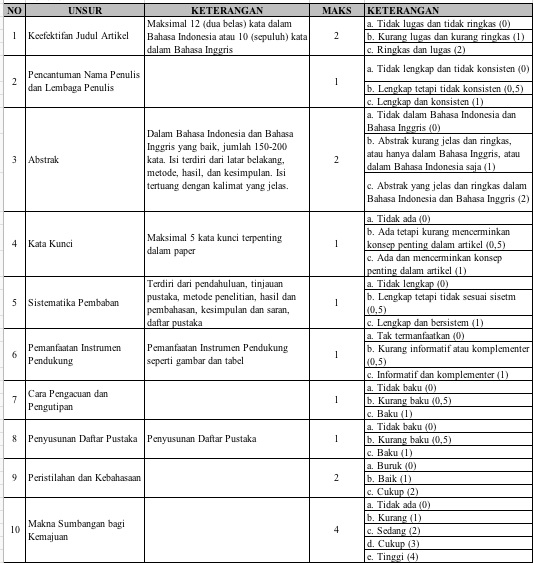
\includegraphics[width=1\textwidth]
      {figures/form1}}
      \caption{Form nilai bagian 1.}
      \label{form1}
      \end{figure}

	\begin{figure}[ht]
	      \centerline{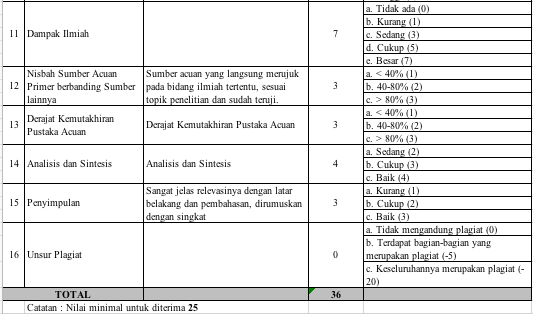
\includegraphics[width=1\textwidth]
	      {figures/form2}}
	      \caption{form nilai bagian 2.}
	      \label{form2}
	      \end{figure}

\chapter{FAQ}

M : Kalo Intership II atau TA harus buat aplikasi ?
D : Ga harus buat aplikasi tapi harus ngoding

M : Pa saya bingung mau ngapain, saya juga bingung mau presentasi apa?
D : Makanya baca de, buka jurnal topik `ganteng' nah kamu baca dulu sehari 5 kali ya, 4 hari udah 20 tuh. Bingung itu tanda kurang wawasan alias kurang baca.

M : Pa saya sudah cari jurnal terindeks scopus tapi ga nemu.
D : Kamu punya mata de? coba dicolok dulu. Kamu udah lakuin apa aja? tolong di list laporkan ke grup Tingkat Akhir. Tinggal buka google scholar klik dari tahun 2014, cek nama jurnalnya di scimagojr.com beres.

M : Pa saya belum dapat tempat intership, jadi ga tau mau presentasi apa?
D : kamu kok ga nyambung, yang dipresentasikan itu yang kamu baca bukan yang akan kamu lakukan.

M : Pa ini jurnal harus yang terindex scopus ga bisa yang lain ?
D : Index scopus menandakan artikel tersebut dalam standar semantik yang mudah dipahami dan dibaca serta bukan artikel asal jadi. Jika diluar scopus biasanya lebih sukar untuk dibaca dan dipahami karena tidak adanya proses review yang baik dan benar terhadap artikel.

M : Pa saya tidak mengerti
D : Coba lihat standar alasan

M : Pa saya bingung
D : Coba lihat standar alasan

M : Pa saya sibuk
D : Mbahmu....

M : Pa saya ganteng
D : Ndasmu....

M : Pa saya kece
D : wes karepmu lah....


Biasanya anda memiliki alasan tertentu jika menghadapi kendala saat proses bimbingan, disini saya akan melakukan standar alasan agar persepsi yang diterima sama dan tidak salah kaprah. Penggunaan kata alasan tersebut antara lain :

1. Tidak Mengerti : anda boleh menggunakan alasan ini jika anda sudah melakukan tahapan membaca dan meresumekan 15 jurnal. Sudah mencoba dan mempraktekkan teorinya dengan mencari di youtube dan google minimal 6 jam sehari selama 3 hari berturut-turut.

2. Bingung : anda boleh mengatakan alasan bingung setelah maksimal dalam berusaha menyelesaikan tugas bimbingan dari dosen(sudah dilakukan semua). Anda belum bisa mengatakan alasan bingung jika anda masih belum menyelesaikan tugas bimbingan dan poin nomor 1 diatas. Setelah anda menyelesaikan tugas bimbingan secara maksimal dan tahap 1 poin diatas, tapi anda masih tetap bingung maka anda boleh memakai alasan ini.

%next line adds the Bibliography to the contents page
\addcontentsline{toc}{chapter}{Bibliography}
%uncomment next line to change bibliography name to references
%\renewcommand{\bibname}{References}
\bibliography{references}        %use a bibtex bibliography file refs.bib
\bibliographystyle{plain}  %use the plain bibliography style

\end{document}

